\documentclass[UTF8]{ctexart}
\usepackage{amsmath}
\usepackage{amssymb}
\usepackage{booktabs}
\usepackage{background}
\usepackage{caption,subcaption}
\usepackage{CJKfntef}
\usepackage{cprotect}
\usepackage{enumitem}
\usepackage{extarrows}
\usepackage{fancyhdr}
\usepackage{float}
\usepackage{fontspec}
%\usepackage{fourier}
\usepackage{geometry}
\usepackage{listings}
\usepackage{tasks}
\usepackage{tcolorbox}
\tcbuselibrary{breakable}
\usepackage{tikz}
\usetikzlibrary{arrows.meta}
\usepackage[table]{xcolor}

\geometry{a5paper, top=0.1cm, left=1cm, right=1cm, bottom=1cm, footskip=0.1cm}
\setCJKmainfont[BoldFont={汉仪文黑-85W},ItalicFont={方正苏新诗柳楷简体}]{汉仪文黑-55W}
\setfontfamily\Issue{Century Schoolbook}
\setfontfamily\Genshin{Genshin Teyvat Lingua Franca}
\newCJKfontfamily\TitleFont{思源宋体 CN Heavy}
\newfontfamily\timesnewroman{Times New Roman}
%\reversemarginpar

\pagestyle{fancy}
\fancyhf{}
%\cfoot{\sffamily\footnotesize{-\ \thepage\ -}} 本次知识小料不使用页码
%\CTEXsetup[format = {\centering\bfseries\large}, beforeskip = 3pt, afterskip = 3pt]{section}

\colorlet{darkcyan}{cyan!50!black}
\newcommand\Black[1]{\textcolor[gray]{0.3}{#1}}
\newcommand\Brown[1]{\textcolor[HTML]{998A4E}{#1}}
\newcommand\Emph[1]{\colorbox{green!10}{\textcolor{green!30!black}{#1}}}
\newcommand\Notes[1]{\textcolor{yellow!50!black}{\small #1}}
\newcommand\Example[1]{\textcolor{cyan!70!black}{\small #1}}
\newcommand\keyword[1]{\textcolor{violet}{\textbf{\texttt{#1}}}}

\newcommand\AND{\  \textrm{AND}\ }
\newcommand\OR{\  \textrm{OR}\ }
\newcommand\IF{\quad\textrm{IF}\quad}
\newcommand\THEN{\quad\textrm{THEN}\quad}
\newcommand\CF{{C\hspace{-0.2em}F}}

\lstset{
    basicstyle=\small\ttfamily, %注意行末有逗号!
    keywordstyle=\bfseries\color{blue!70!black},
    commentstyle=\color{cyan!90!black},
    stringstyle=\color{green!40!black},
    columns=flexible,
    numbers=left,
    numberstyle=\footnotesize,
    escapechar=`,
    frame=shadowbox,
    %rulesepcolor=\color{red!20!blue!20!green!20}
    backgroundcolor=\color{cyan!5!white},
    language = C++,
    tabsize = 4,
    breaklines = true,
    showstringspaces = false,
}

\newcommand\IssueNumber{36}
\newcommand\Date{2024-10-12}
%\newcommand\Contributer{@金光日}
\newcommand\Subject{计算机网络}


\begin{document}
\backgroundsetup{contents=
\includegraphics{上半示例.png}, center, scale=1, angle=0, opacity=1}
\BgThispage
\begin{center}
%{\scriptsize\Issue \textcolor[HTML]{C8BA83}{\Genshin WEEKLY TIPS}}
\phantom{...}

{\Large\textcolor{brown!40!white}{\makebox[10cm][s]{\Genshin WEEKLY KNOWLEDGE TIPS}}}

\vspace{-2em}

{\Huge\bfseries\TitleFont \Black{知\ 识\ 小\ 料}}


\vspace{-0.1cm}
{\footnotesize \Brown{「电计 2203 班」周常规知识整理共享}}
\end{center}

\vspace{-0.5cm}


\begin{figure}[H]
\hspace{1cm}
\begin{minipage}[t]{0.3\textwidth}
\centering
    \Brown{\Genshin ISSUE}

    \vspace{-0.6cm}
    \Huge \Issue\slshape\bfseries\Black{\IssueNumber}
\end{minipage}
\hfill
\begin{minipage}[t]{0.35\textwidth}
\centering
    \Brown{日期:\Date} \\
%\vspace{-0.1cm}
%    \Brown{贡献者:\Contributer} \\
\vspace{-0.1cm}
    \Brown{学科:\Subject} \\
\end{minipage}
\hspace{0.8cm}
\end{figure}

{\color{cyan!50!black}
\begin{enumerate}
  \item 若甲向乙发起了一条 TCP 的连接,最大段长为 1KB,乙每收到一个数据段都会发出一个接收窗口为 10KB 的确认段,若甲在 $t$ 时刻发生超时,此时拥塞窗口为 16KB。则从 $t$ 时刻起,在不再发生超时的情况下,经过 10 个 RTT 后,甲的发送窗口是

      A. 10KB \hfill B. 12KB \hfill C. 14KB \hfill D. 15KB \hfill

  \item 一个 TCP 连接总以 1KB 的最大段长发送 TCP 段,发送方有足够多的数据要发送,当拥塞窗口为 16KB 时发生了超时,若接下来的 4 个 RTT 时间内的 TCP 段的传输都是成功的,则当第 4 个 RTT 时间内发送的所有 TCP 段都得到肯定应答时,拥塞窗口大小是

      A. 7KB \hfill B. 8KB \hfill C. 9KB \hfill D. 16KB \hfill
\end{enumerate}
}

答案见下页……

\newpage

\paragraph{【问题 1】}
$t$ 时刻超时,慢开始门限 ssthresh 取 8KB(拥塞窗口的一半)。此后,拥塞窗口的大小在 1 个 RTT 后重设为 1,相继采用慢开始和拥塞避免算法:
\begin{itemize}[itemsep=0pt,parsep=0pt]
  \item 小于门限则指数增长,不断乘 2;
  \item 大于等于门限则线性增长,不断加 1KB(即最大段长 MSS)。
\end{itemize}

\begin{figure}[htb]
    \centering
    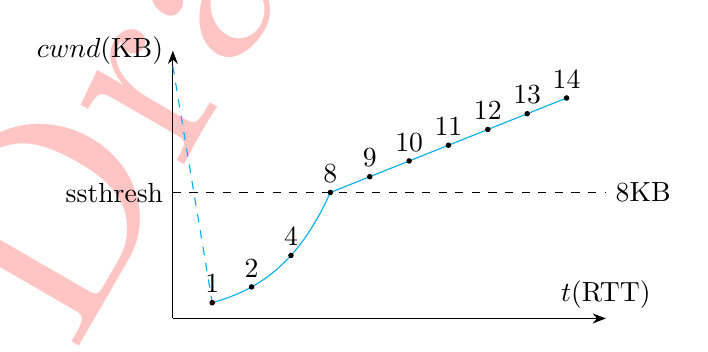
\begin{tikzpicture}[>=Stealth,xscale=0.5, yscale=0.2]
        \draw[->] (0,0) -- (11,0) node[above] {$t$(RTT)};
        \draw[->] (0,0) -- (0,17) node[left] {$cwnd$(KB)};
        \draw[dashed] (0,8) node[left] {ssthresh} -- (11,8) node[right] {8KB} ;
        \draw[cyan, dashed] (0,16) -- (1,1);
        \draw[cyan, domain = 1:4] plot (\x, 0.5*2^\x); % y = 2^(x+1)
        \draw[cyan] (4,8) -- (10,14);
        \fill (1,1) circle [x radius=2pt, y radius=5pt] node[above] {1};
        \fill (2,2) circle [x radius=2pt, y radius=5pt] node[above] {2};
        \fill (3,4) circle [x radius=2pt, y radius=5pt] node[above] {4};
        \fill (4,8) circle [x radius=2pt, y radius=5pt] node[above] {8};
        \foreach \i in {9,10,...,14}{
            \fill (\i-4, \i) circle [x radius=2pt, y radius=5pt] node[above] {\i};
        }
    \end{tikzpicture}
    \caption{形象地理解拥塞窗口增加的过程}\label{fig:1}
\end{figure}
因此,在 $1,2,\dots,10$ 个 RTT 时拥塞窗口依次为:$1,2,4,8,9,10,11,12,13,14$(KB)。

这时候选 C?那就错啦!因为题目问的是\textbf{发送窗口},它应该取接收窗口和拥塞窗口的\textbf{最小值},所以答案是 10KB,选 A。

\backgroundsetup{contents=
\includegraphics{下半示例.png}, center, scale=1, angle=0, opacity=1}
\BgThispage
\paragraph{【问题 2】}
超时以后,慢开始门限 ssthresh 取 8KB(拥塞窗口的一半)。此后,按慢开始算法,拥塞窗口的大小在 $1,2,3,4$ 个 RTT 依次为:$1,2,4,8$(KB),看起来似乎如此。

但是,因为题目问的是 4 个 RTT 时间内\textbf{传输都是成功的},而 $cwnd$ 从 $16$ 变成 $1$ 的那一个 RTT 正处于超时阶段,没有传输成功,所以应该从 $cwnd=1$ 的时候开始算 RTT。如此一来,经过 $1,2,3,4$ 个 RTT 后依次为 $2,4,8,9$(KB)。

在第 4 个 RTT 发送的包得到肯定应答的时候,拥塞窗口为 9KB。选 C。


\vspace{1em}
{\color{cyan!80!black}
【结论】1. A; 2. C。

【点评】这是两道计网的考研相关题,其中第二道是 2009 年的真题。考察的是 TCP 的拥塞窗口的相关知识,比较坑,需要同学们多多留意。
}

\end{document} 